\section{Product perspesctive}
\label{sec:product_perspesctive}%

\subsection{Scenarios}
\label{subsec:scenarios}%
\paragraph{Scenario 1: A student registers}
A university student named \textbf{Amelia Young} chooses to work for S\&C while searching for an internship. After accessing the platform's home page, she selects the \textbf{"Sign-Up"} option and inputs her email address, name, and a strong password. She gets a confirmation email after completing the form. Amelia activates her account by clicking on the confirmation link. After finishing, she logs on to look for internship possibilities.

\paragraph{Scenario 2: A Company posts an internship}
Interns are needed for the data analytics team at \textbf{InnovateCorp}, a mid-sized software startup. After logging in to S\&C, an HR representative from the organization fills out the \textbf{"Post Internship"} part, which includes the job title, description, length, and needed qualifications. They also establish a deadline for applications. After submission, S\&C gives InnovateCorp a confirmation email and contacts the appropriate students based on their profiles.

\paragraph{Scenario 3: A University administrator monitors internships}
\textbf{Greenfield University} academic coordinator \textbf{Dr. Olivia Cruz} uses S\&C to monitor the development of her students' internships. She goes to the \textbf{"Internship Monitoring"} section, where she may see comprehensive reports, examine student and company comments, and respond to complaints made by either side.
 

\paragraph{Scenario 4: A Student applies for an internship}
\textbf{Liam Chen}, a computer science major, looks for software development internships on S\&C. He discovers a position at InnovateCorp that suits him after using filters to refine the results. After reading the job description, Liam selects \textbf{"Apply Now"} and sends in his resume. On his dashboard, the application status is updated.

\paragraph{Scenario 5: A Company reviews applications}
Notifications of new applications are sent to InnovateCorp's HR department. They access Liam's profile and resume by logging in to the \textbf{"Application Management"} area. Following screening, Liam is placed on their shortlist, and his dashboard is automatically updated with the interview time.

\subsection{System Context}
The Students \& Companies (S\&C) platform is a dynamic web-based solution designed to streamline the internship process by bridging the gap between students, companies, and universities. The platform caters to three primary user groups, each with distinct roles and requirements:

\begin{enumerate}
    \item \textbf{University Students:} Students utilize the platform to search for internship opportunities, create detailed profiles with CVs and skills, and track their application progress.
    \item \textbf{Companies:} Organizations post internship positions, outline role requirements, and select suitable candidates based on student profiles and recommendations.
    \item \textbf{University Administrators:}
    Universities leverage the platform to oversee the entire internship process, monitor student performance, and ensure alignment with academic standards.
    \item \textbf{Central Platform:} The S\&C platform serves as a centralized hub, fostering efficient communication, reducing administrative overhead, and ensuring a seamless experience for all stakeholders involved.
\end{enumerate}

\newpage

\subsection{Class diagrams}
\label{subsec:class_diagrams}%


\begin{figure}[H]
    \begin{center}
        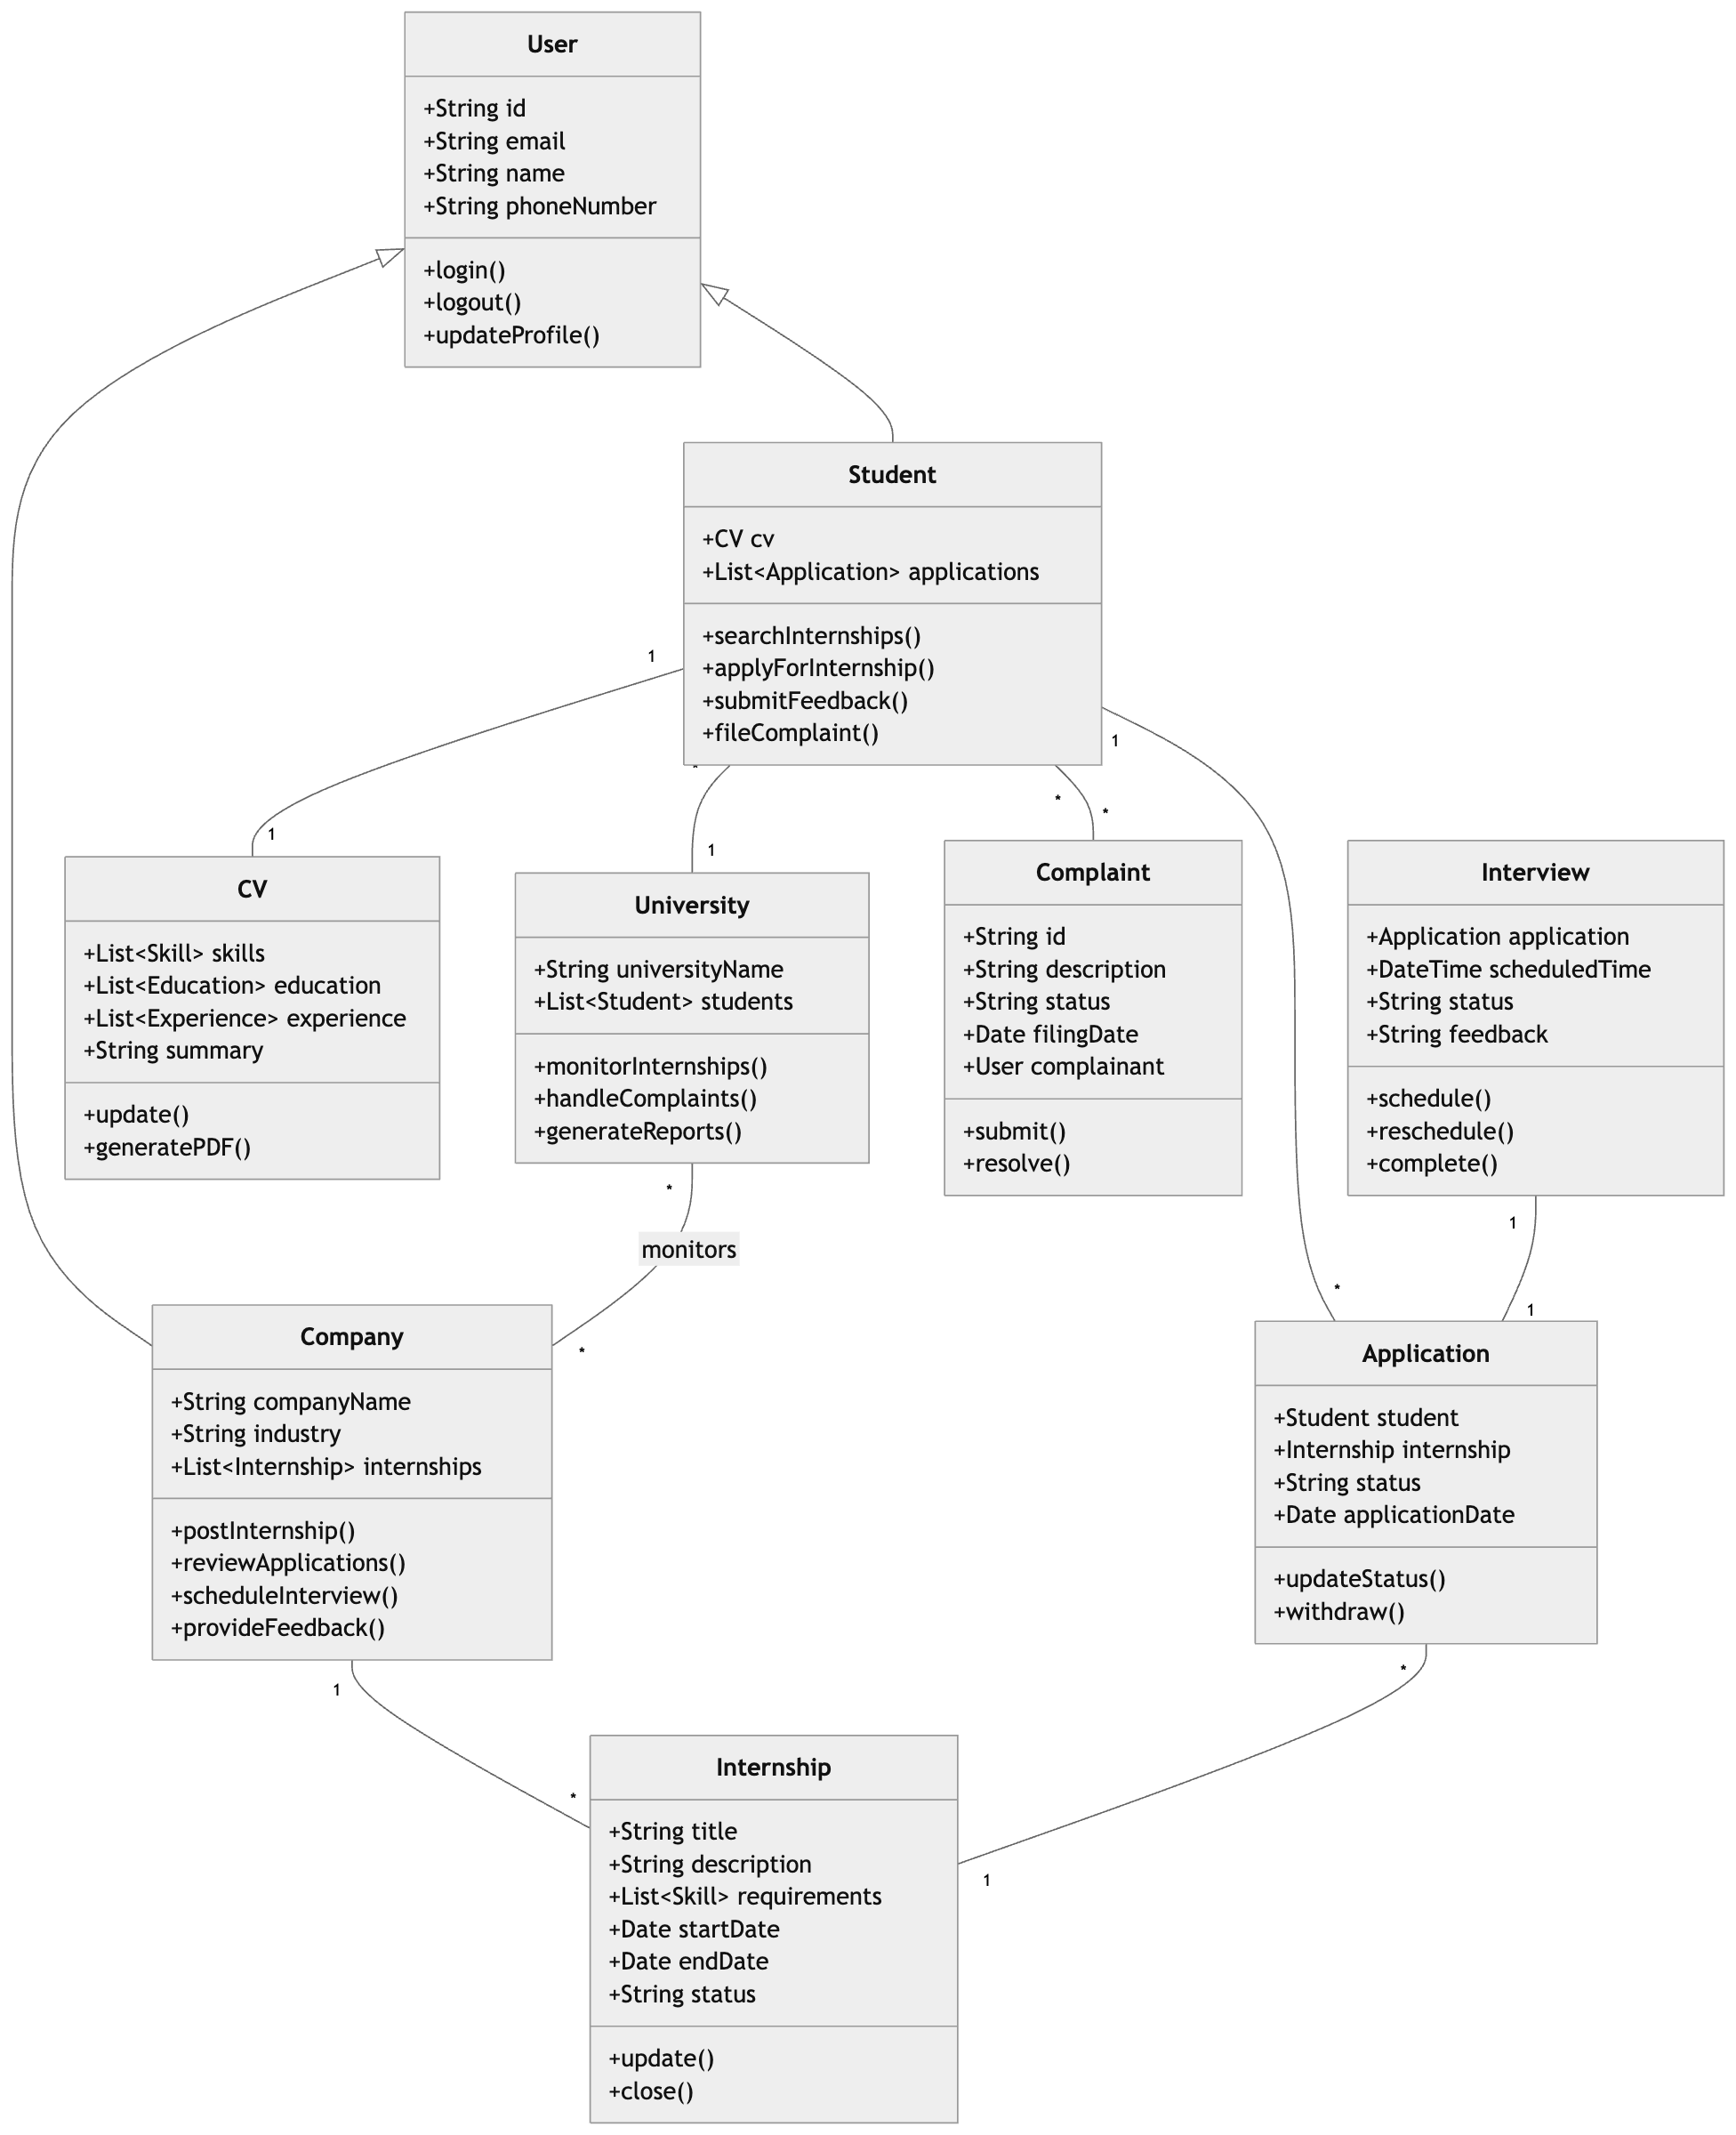
\includegraphics[width=0.9\linewidth]{JhaBhatiaSharma/Images/InternHubClassDiagram.png}
        \caption{Class Diagram for InternHub}
        \label{fig:UML}%
    \end{center}
\end{figure}

The system's core is the \textbf{User class}, which contains shared methods like \textbf{login(), logout(), and updateProfile()} as well as common attributes like id, email, name, and phoneNumber. The User class is extended by specialized classes like Student, University, and Company, each of which adds unique characteristics and features. Students can look for internships, apply, provide feedback, and file complaints using the CV and application list included in the Student class. In the meantime, the University class uses functions like \textbf{monitorInternships() and generateReports()} to handle complaints, internships, and students. Employer-specific tasks like advertising internships, evaluating applications, setting up interviews, and giving feedback are made easier by the Company class.
\par
Auxiliary classes such as Internship, which represents internship details, and Application, which links students to internships and tracks their status, support these core entities. The CV class creates professional resumes by combining a student's education, experience, and skills. To ensure smooth operations, the Complaint and Interview classes oversee the complaint lifecycle and interview procedures, respectively. Each class plays a unique role in the platform's workflow, ensuring scalability and promoting effective communication between businesses, universities, and students.


\subsection{System Architecture}

The platform consists of:

The following elements make up the modular architecture of the S\&C platform:

\begin{enumerate}
    \item \textbf{Front-End Layer:}
    \begin{itemize}
        \item \textbf{Student Portal:} A place where students can track applications, maintain profiles, and search for internships.
        \item \textbf{Company Portal:} Resources for employers to advertise openings, evaluate applicants, and provide feedback.
        \item \textbf{University Administrator Portal:} An interface enabling colleges to manage reports and monitor internships.
        \item \textbf{Public Interface:} Allows users to explore internships and learn more about the platform.
    \end{itemize}
    
    \item \textbf{Services for the Backend:}
    \begin{itemize}
        \item Suggestion for a User Management Service.
        \item Matching Engine.
        \item Recommendation System.
        \item Interview Management Service.
        \item External Integrations for the Service Analytics Engine.
    \end{itemize}
    
    \item \textbf{Email Support:}
    \begin{itemize}
        \item Authentication Service for Document Storage Systems.
        \item Processing payments for compensated internships.
        \item Authentication Service.
        \item Payment Processing (for paid internships).
    \end{itemize}
\end{enumerate}

\begin{figure}[H]
    \begin{center}
        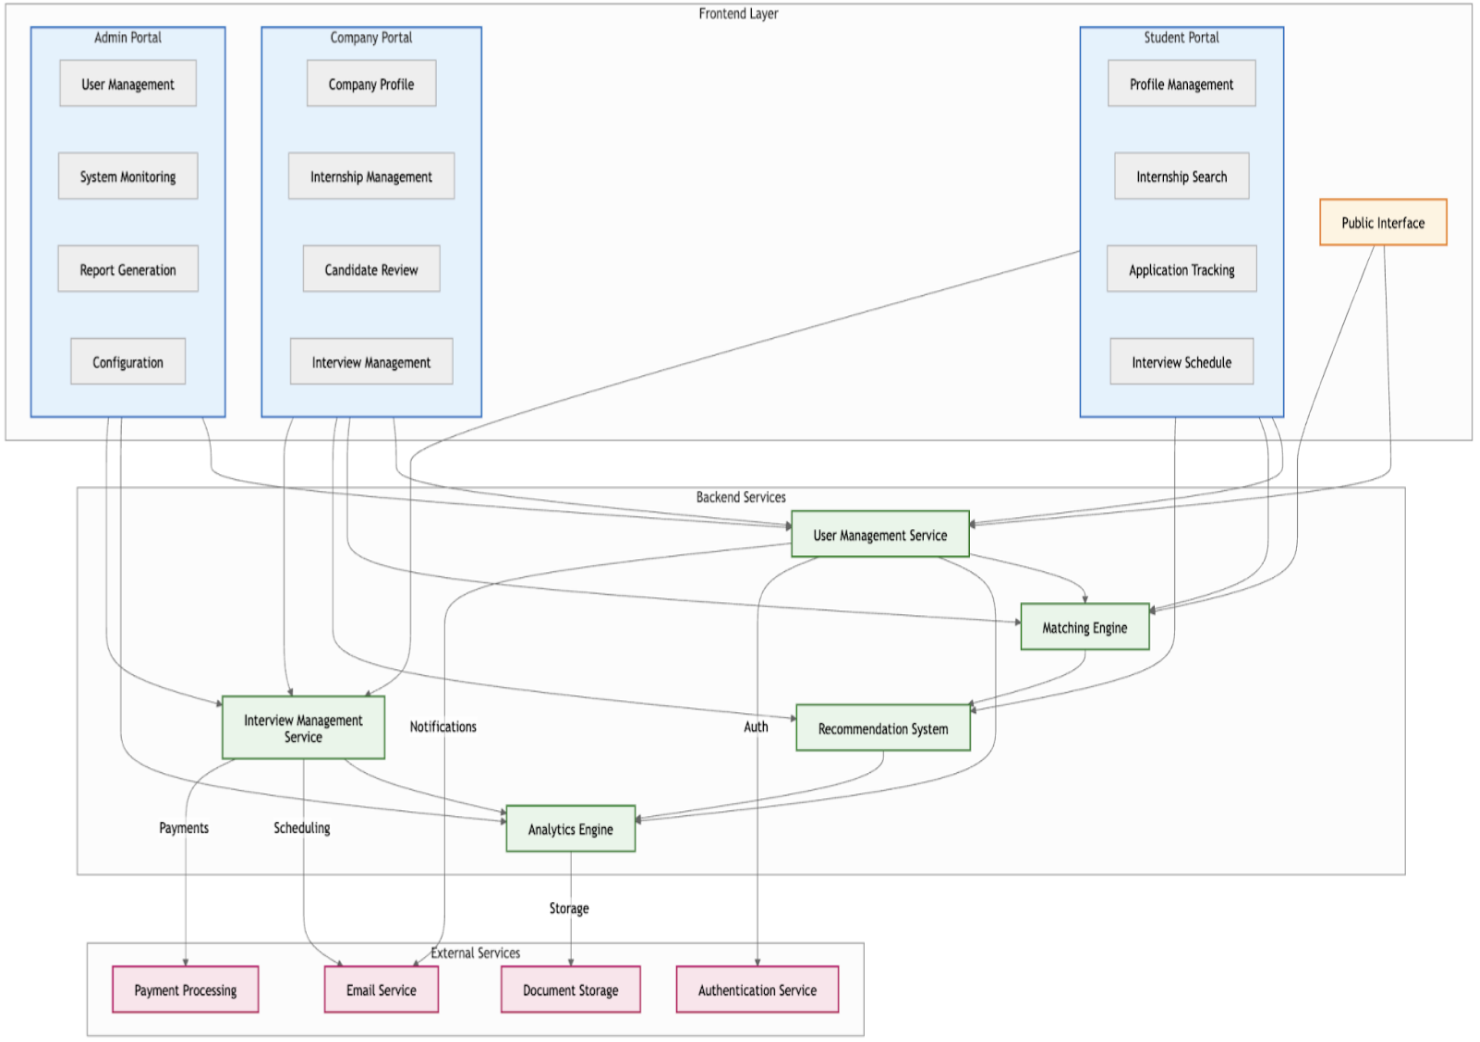
\includegraphics[width=0.9\linewidth]{JhaBhatiaSharma/Images/systemArchitecture.png}
        \caption{System Architecture Diagram for InternHub}
        \label{fig:SysArchitecture}%
    \end{center}
\end{figure}

\subsection{State diagrams}
\label{subsec:state_diagrams}%
The State Diagrams of the S\&C system, which depict every action a user could take, are shown in this section.

\paragraph{SignUp:}
When a user wants to register on S\&C, they must fill out a registration form with their email address, password, name, and last name. S\&C will send the user a verification email if the credentials they have provided are accepted (that is, if the password satisfies security requirements and the email address is not already in use). The new account is successfully created after the user confirms their registration using the email link that was provided. S\&C displays an error notice to the user and reroutes them to the signup form page if the credentials are incorrect.

Additionally, S\&C will ask for more company-specific details including the company name, industry, and size if the user chooses the "Register as a Company" option during the registration process. To construct a comprehensive company profile, these details are necessary.


\begin{figure}[H]
    \begin{center}
        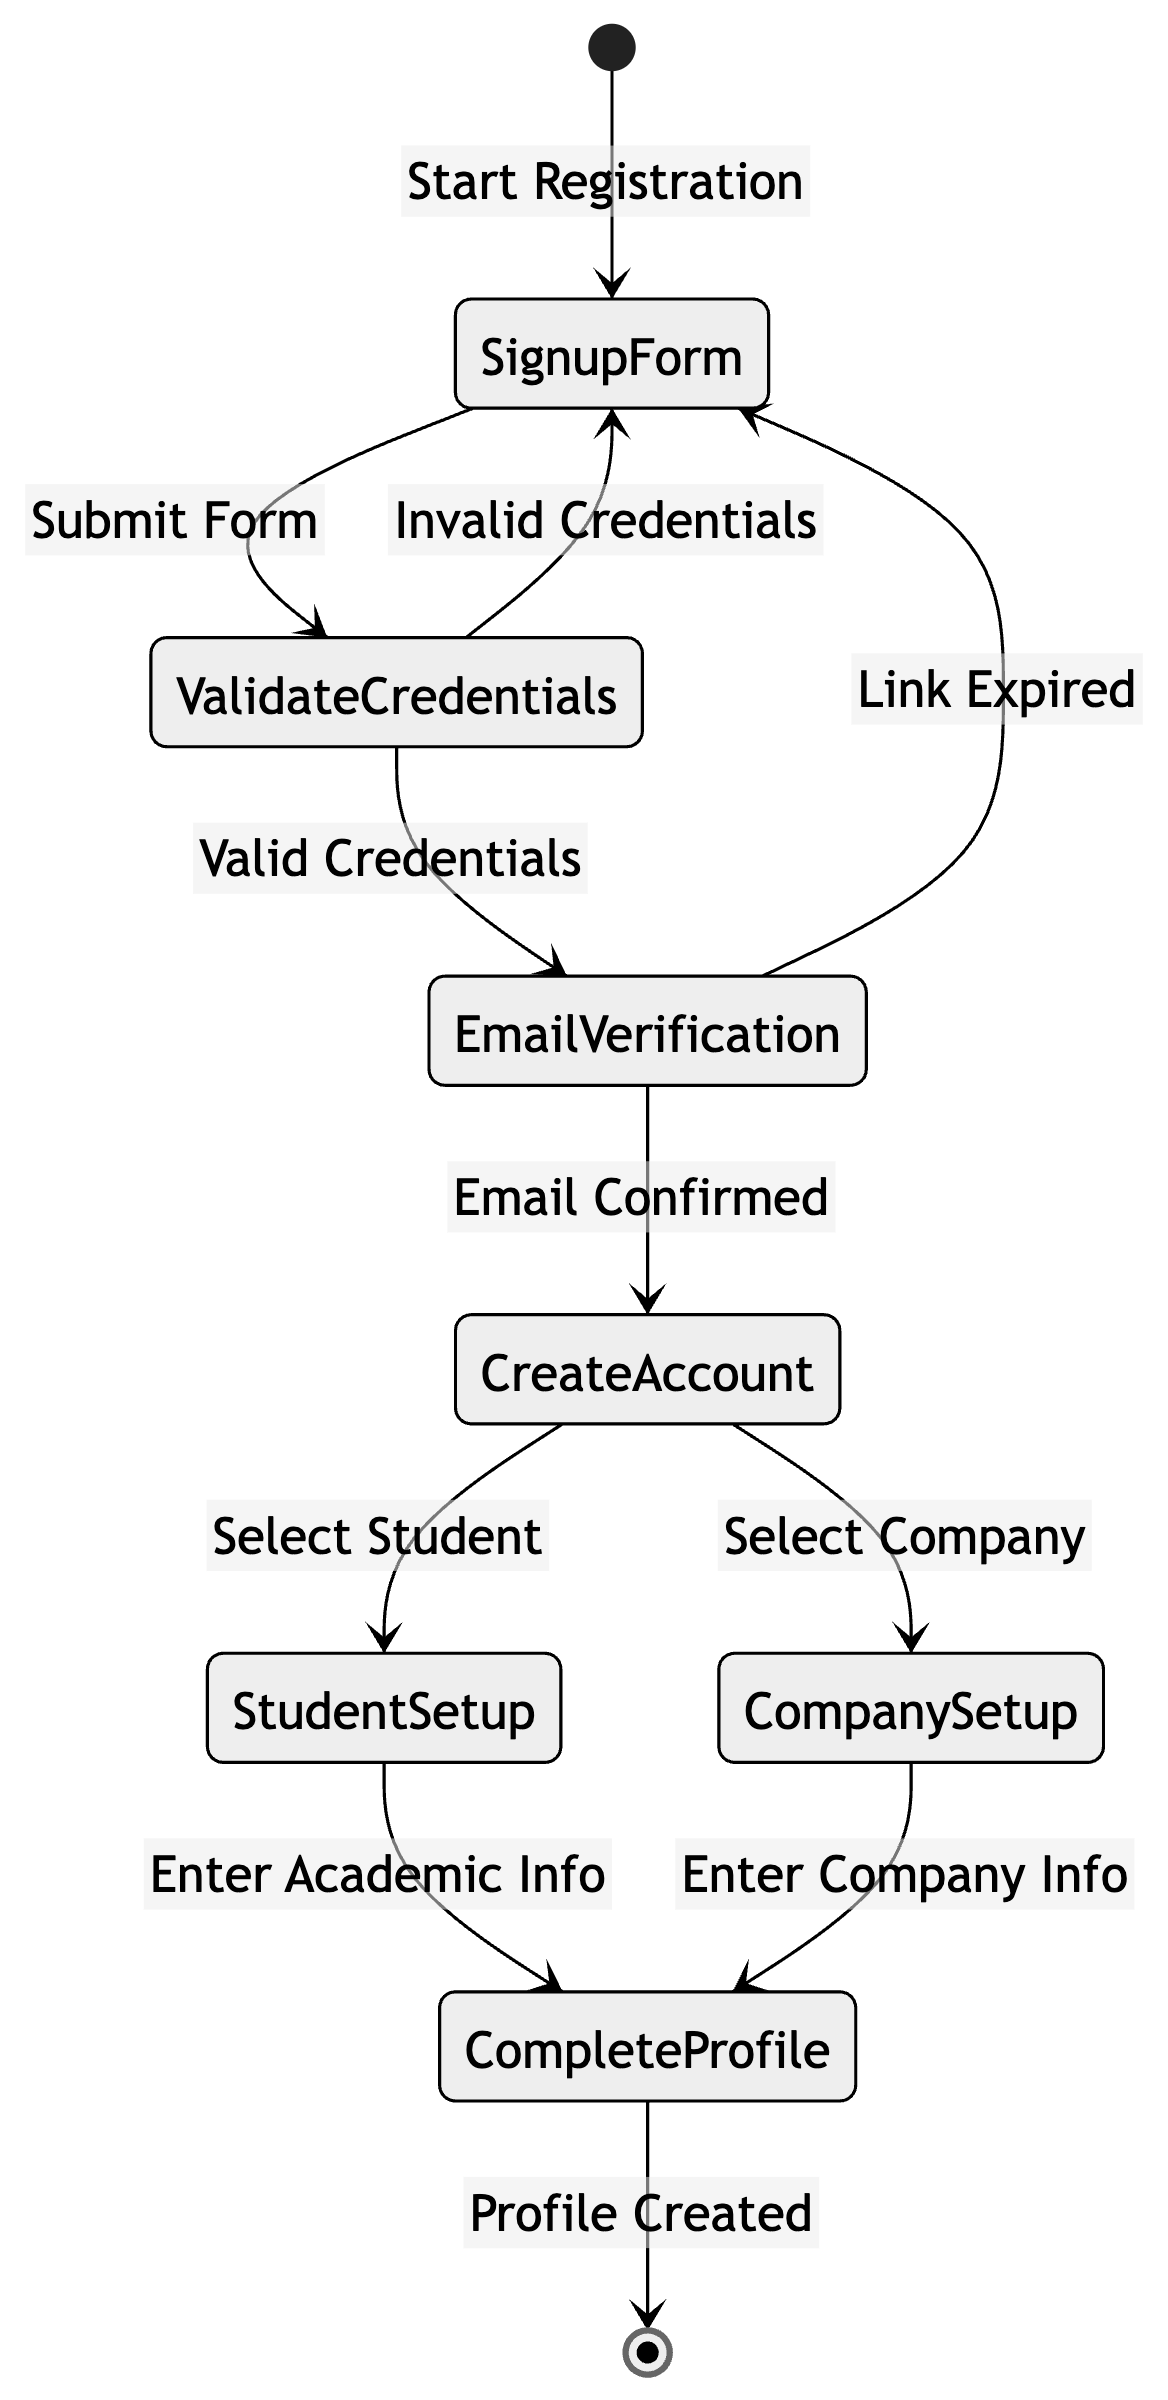
\includegraphics[width=0.5\linewidth]{JhaBhatiaSharma/Images/State Diagrams/SignUp.png}
        \caption{Signup state diagram.}
        \label{fig:signup_sd}%
    \end{center}
\end{figure}

\paragraph{Login:}
A registered user must fill out a login form using their email address and password in order to access their S\&C account. S\&C presents the User's dashboard, which highlights pertinent internships and applications according to their function, if the credentials supplied are correct and correspond to those of a registered User in the S\&C database. S\&C returns the user to the login form page after displaying an error notice if the credentials entered are incorrect.


\begin{figure}[H]
    \begin{center}
        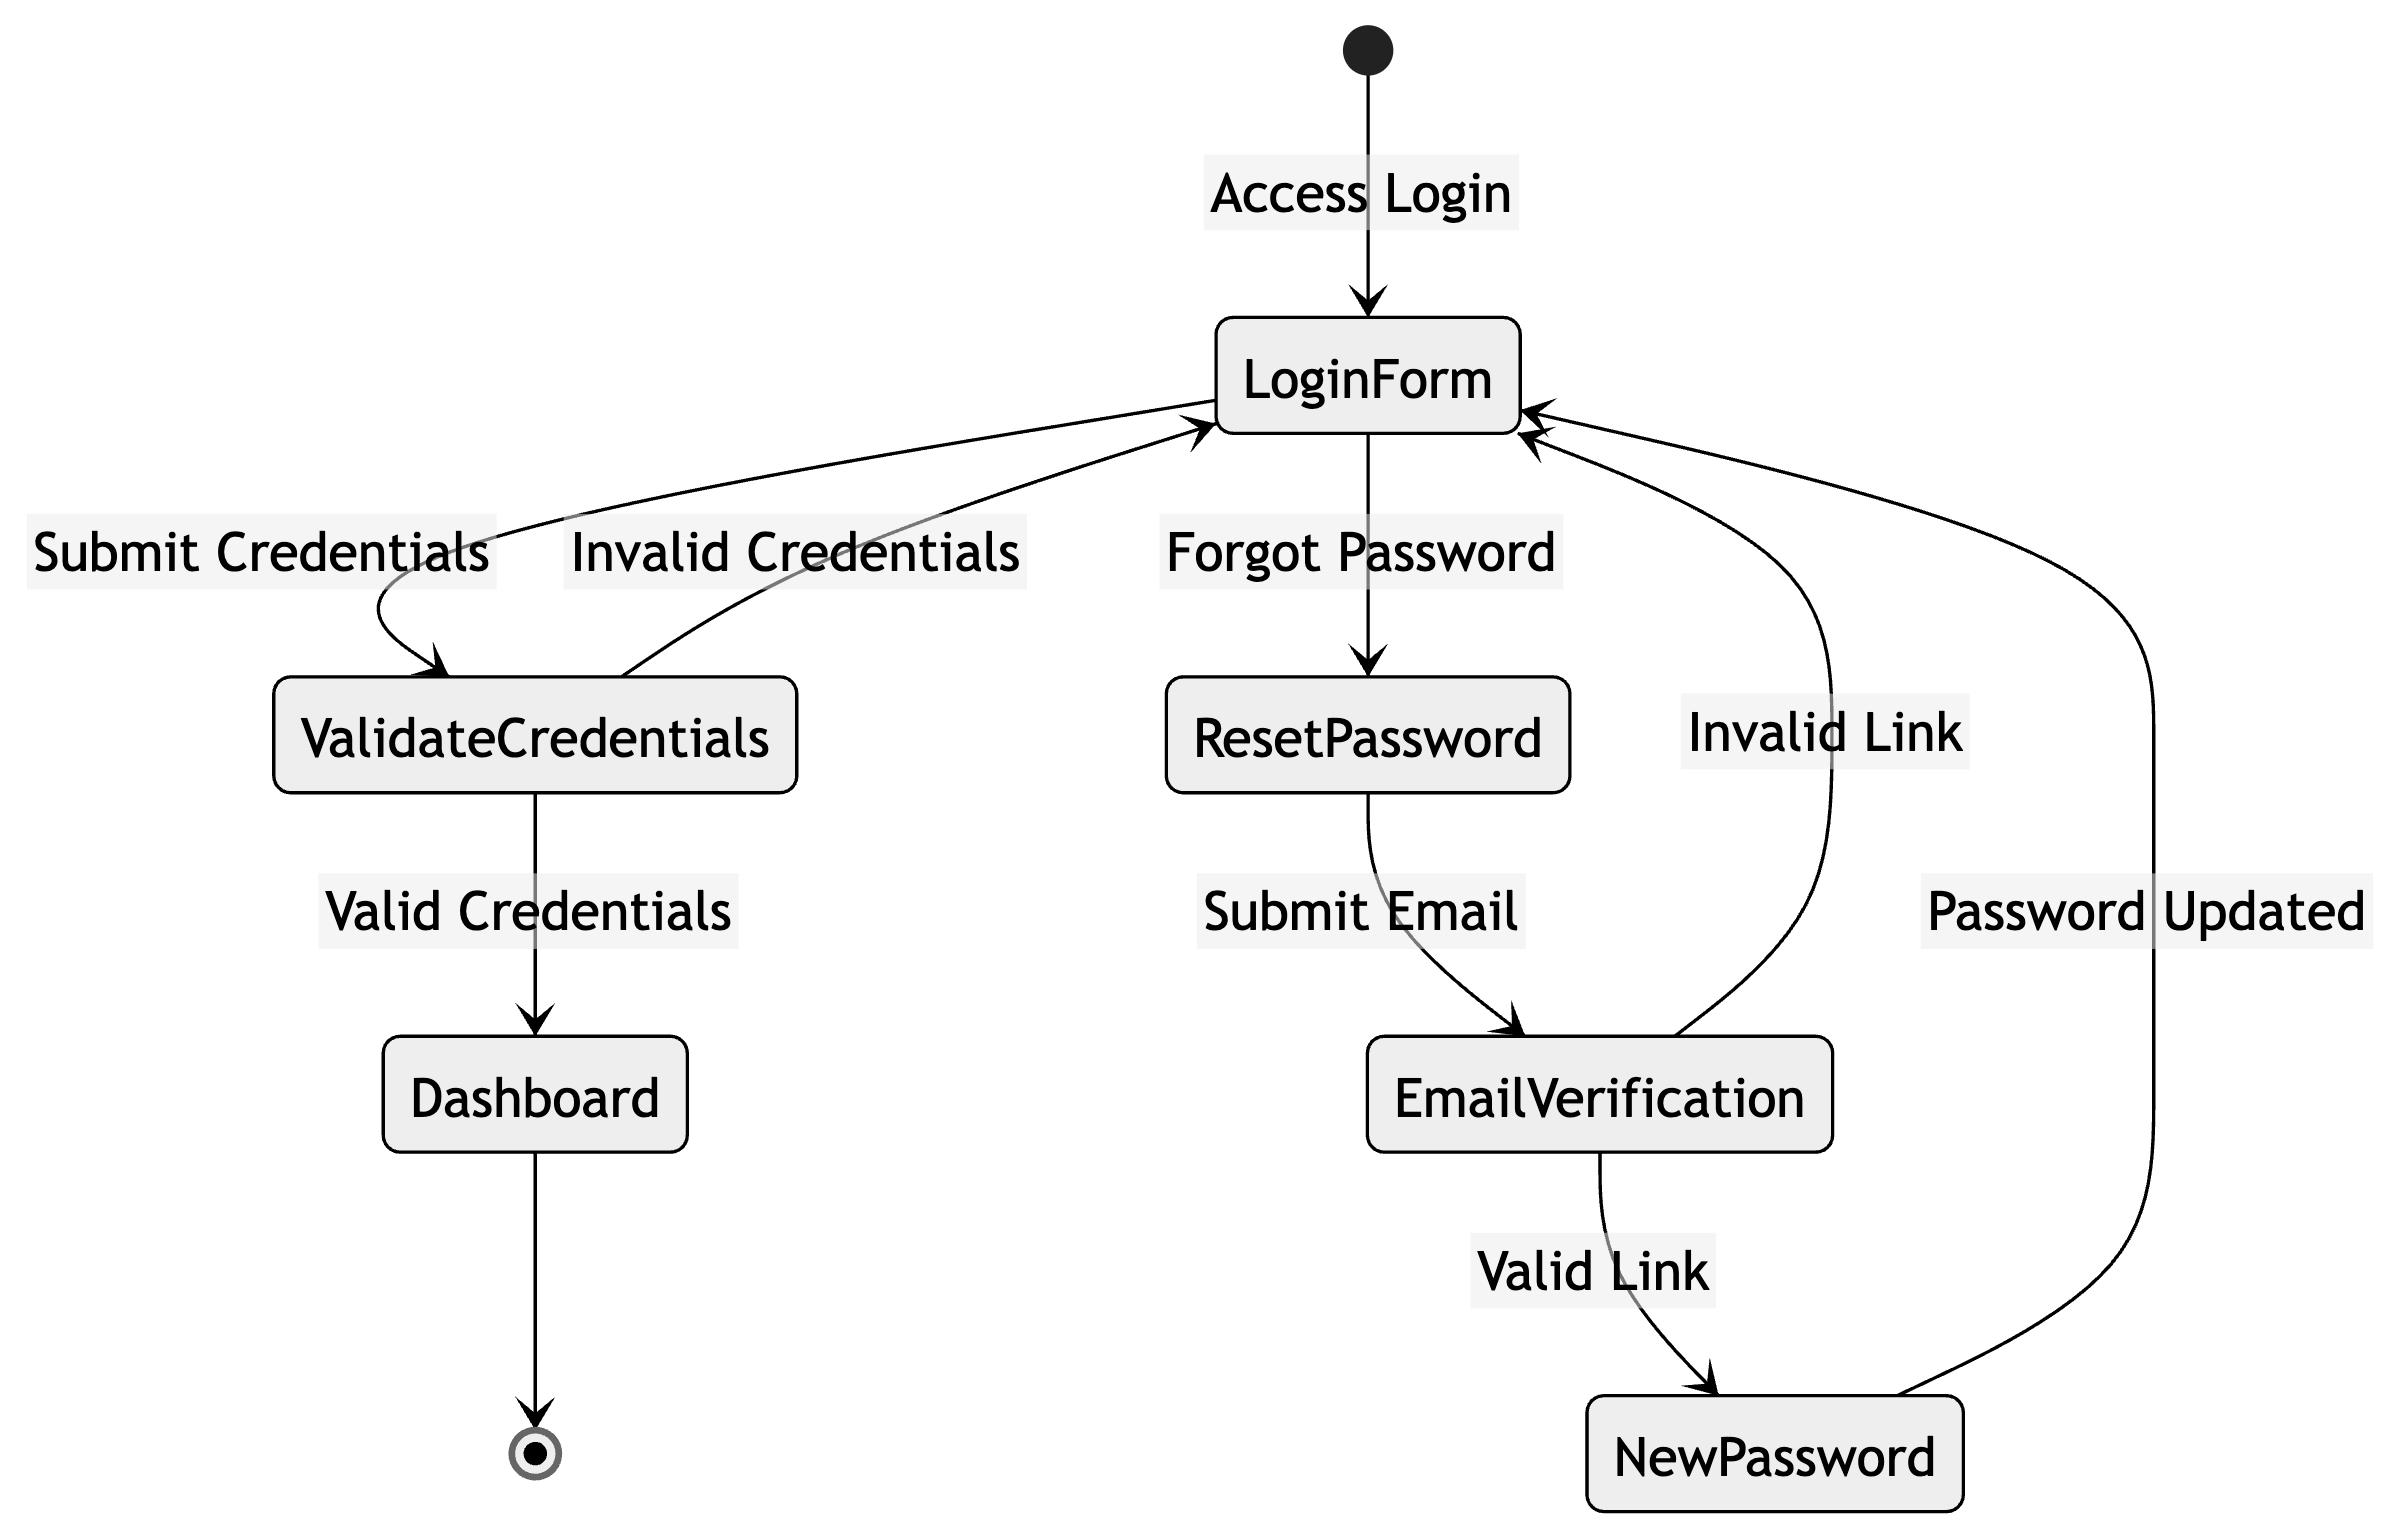
\includegraphics[width=1\linewidth]{JhaBhatiaSharma/Images/State Diagrams/LoginState.png}
        \caption{Login state diagram.}
        \label{fig:login_sd}%
    \end{center}
\end{figure}

\newpage

\paragraph{Post Internship:}
Companies must include a number of parameters in the create internship form when they plan to post a new internship on S\&C. The job title, description, requirements, length of service, and any other information, such pay or perks, are examples of these factors. S\&C shows the Company an error message and reroutes them back to the creation form if the system determines that any of these parameters are inappropriate.
On the other hand, S\&C creates the internship posting if every parameter satisfies the system's requirements. Notifications are subsequently delivered to matching students based on their profiles and preferences after the newly produced posting is published to the Company's dashboard.

\begin{figure}[H]
    \begin{center}
        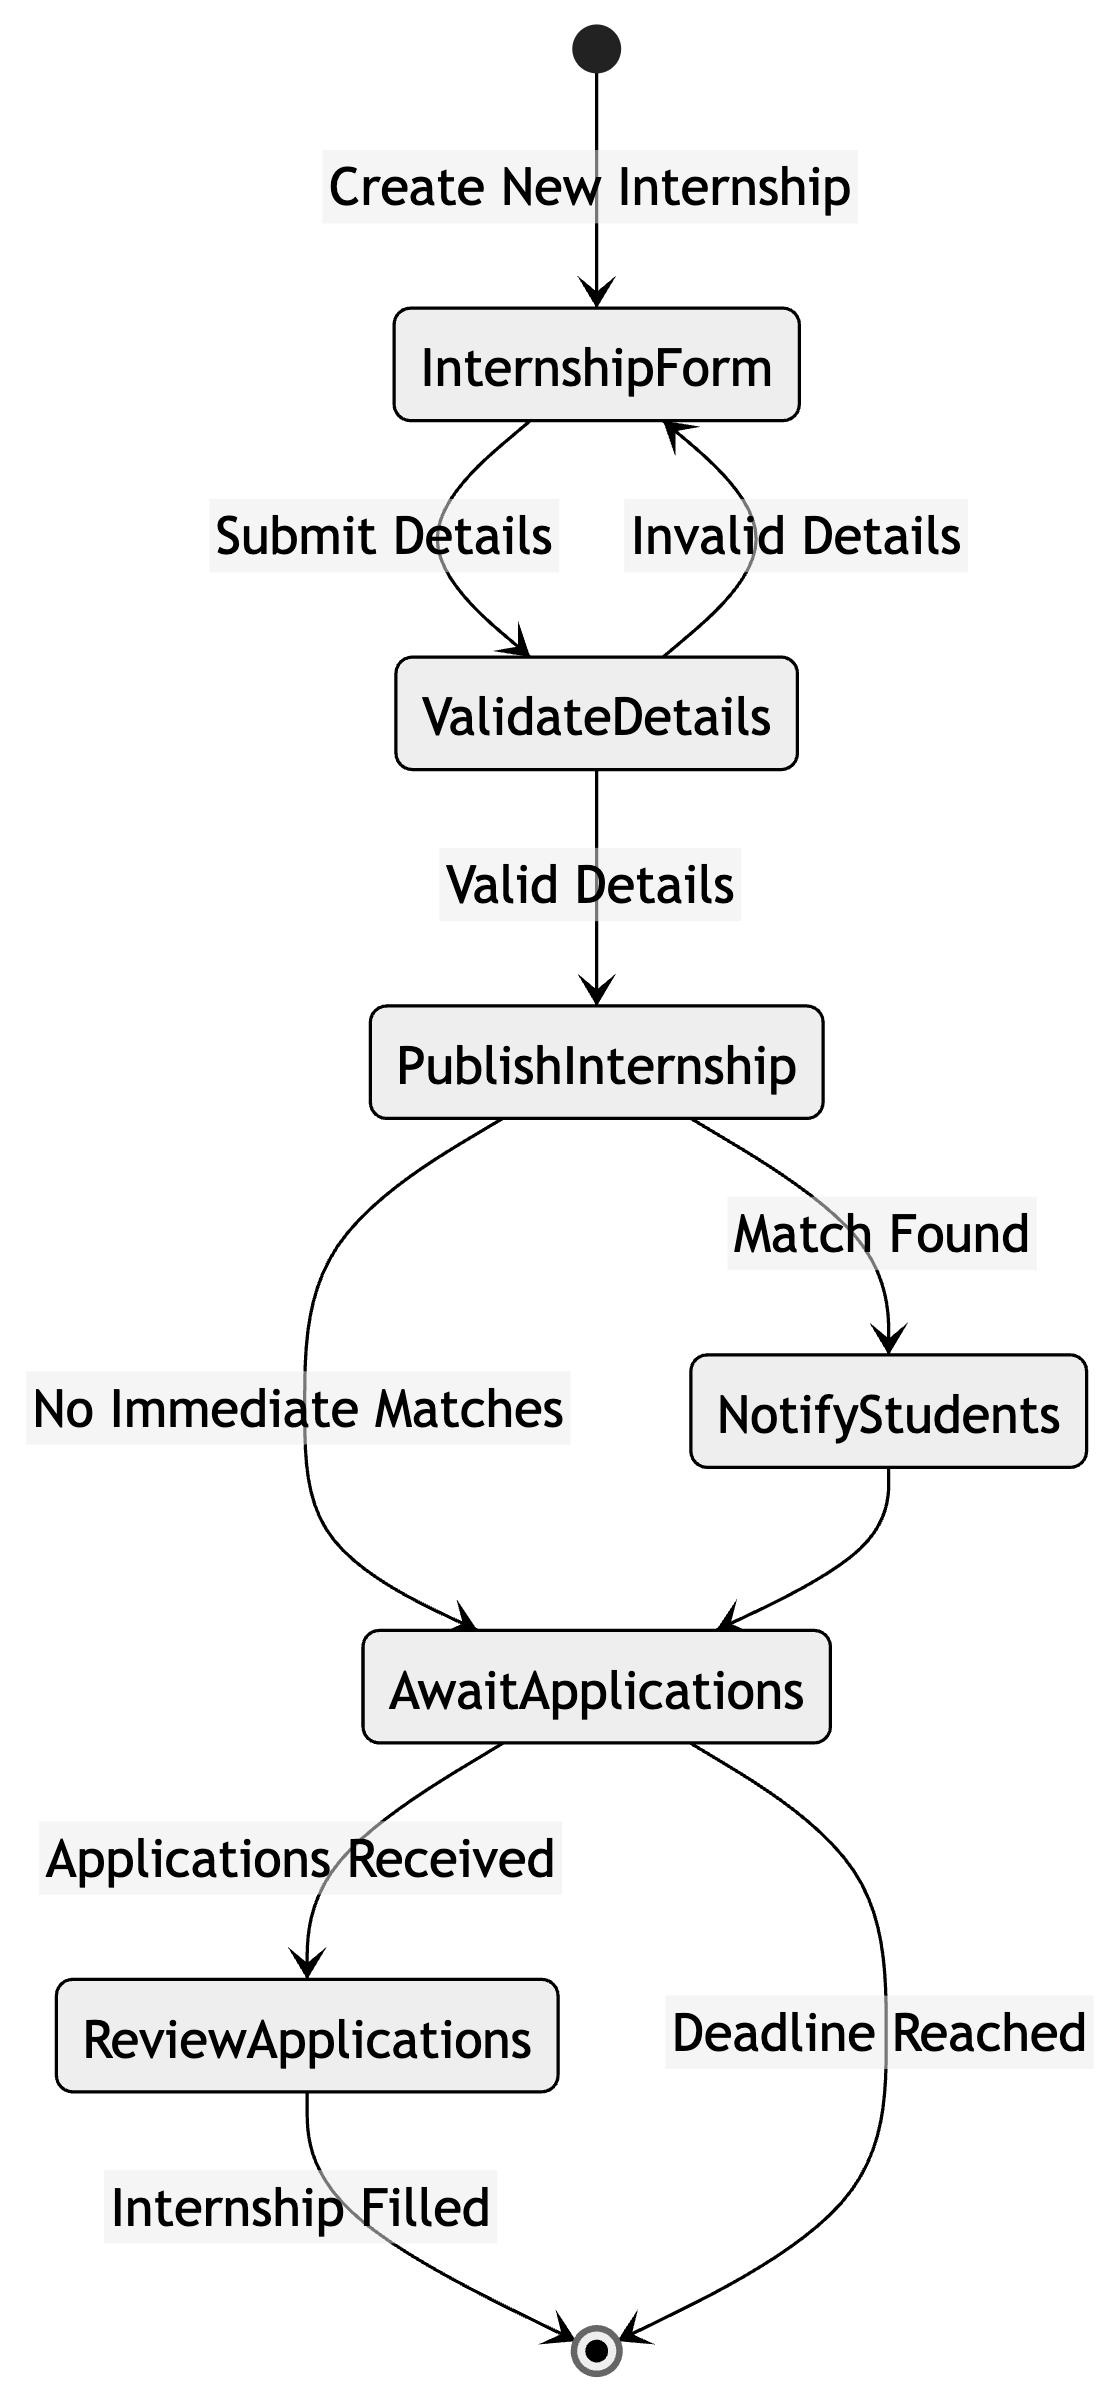
\includegraphics[width=0.35\linewidth]{JhaBhatiaSharma/Images/State Diagrams/PostInternship.png}
        \caption{State Diagram for Post Internship}
        \label{fig:postInternship}%
    \end{center}
\end{figure}

\paragraph{Apply for Internship:}
Students can use the platform to apply for internships when they locate one that interests them. The application form, which could contain extra questions unique to the role, must be filled out by the student. S\&C confirms that the student satisfies the prerequisites and that the application is complete. The application is sent to the business if it is accepted, and the student can monitor its progress via their dashboard. S\&C lets the student finish the application after displaying an error message if any necessary information is lacking.


\begin{figure}[H]
    \begin{center}
        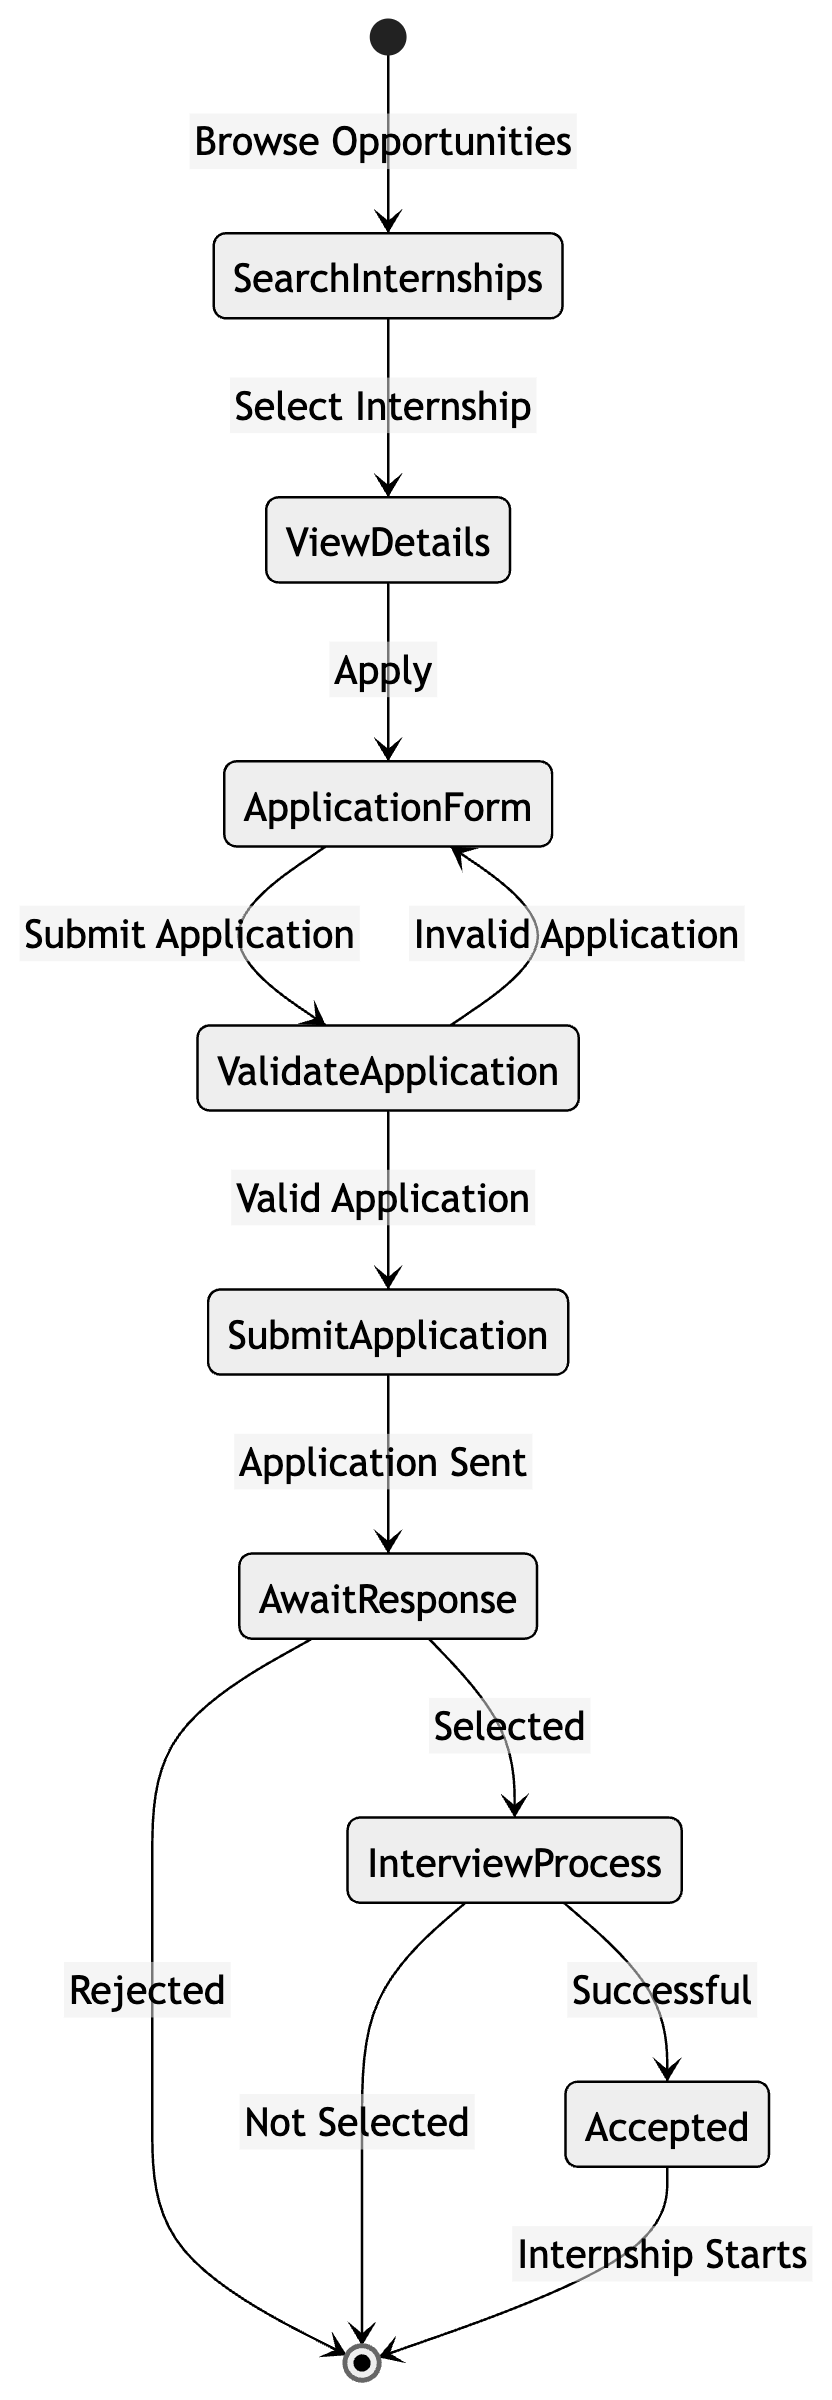
\includegraphics[width=0.35\linewidth]{JhaBhatiaSharma/Images/State Diagrams/ApplyingInternship.png}
        \caption{State Diagram for Applying for an Internship}
        \label{fig:create_Battle_sd}%
    \end{center}
\end{figure}

\paragraph{Interview Management:}
A business can use S\&C to start the interview process after reviewing applications and choosing applicants for interviews. The candidate is informed of the time slots that are available once the organization makes a selection. Other times can be suggested or accepted by the student. Notifications and calendar invitations are sent to both parties after confirmation. Following the interview, the business can document the results and move on with its choice.

\begin{figure}[H]
    \begin{center}
        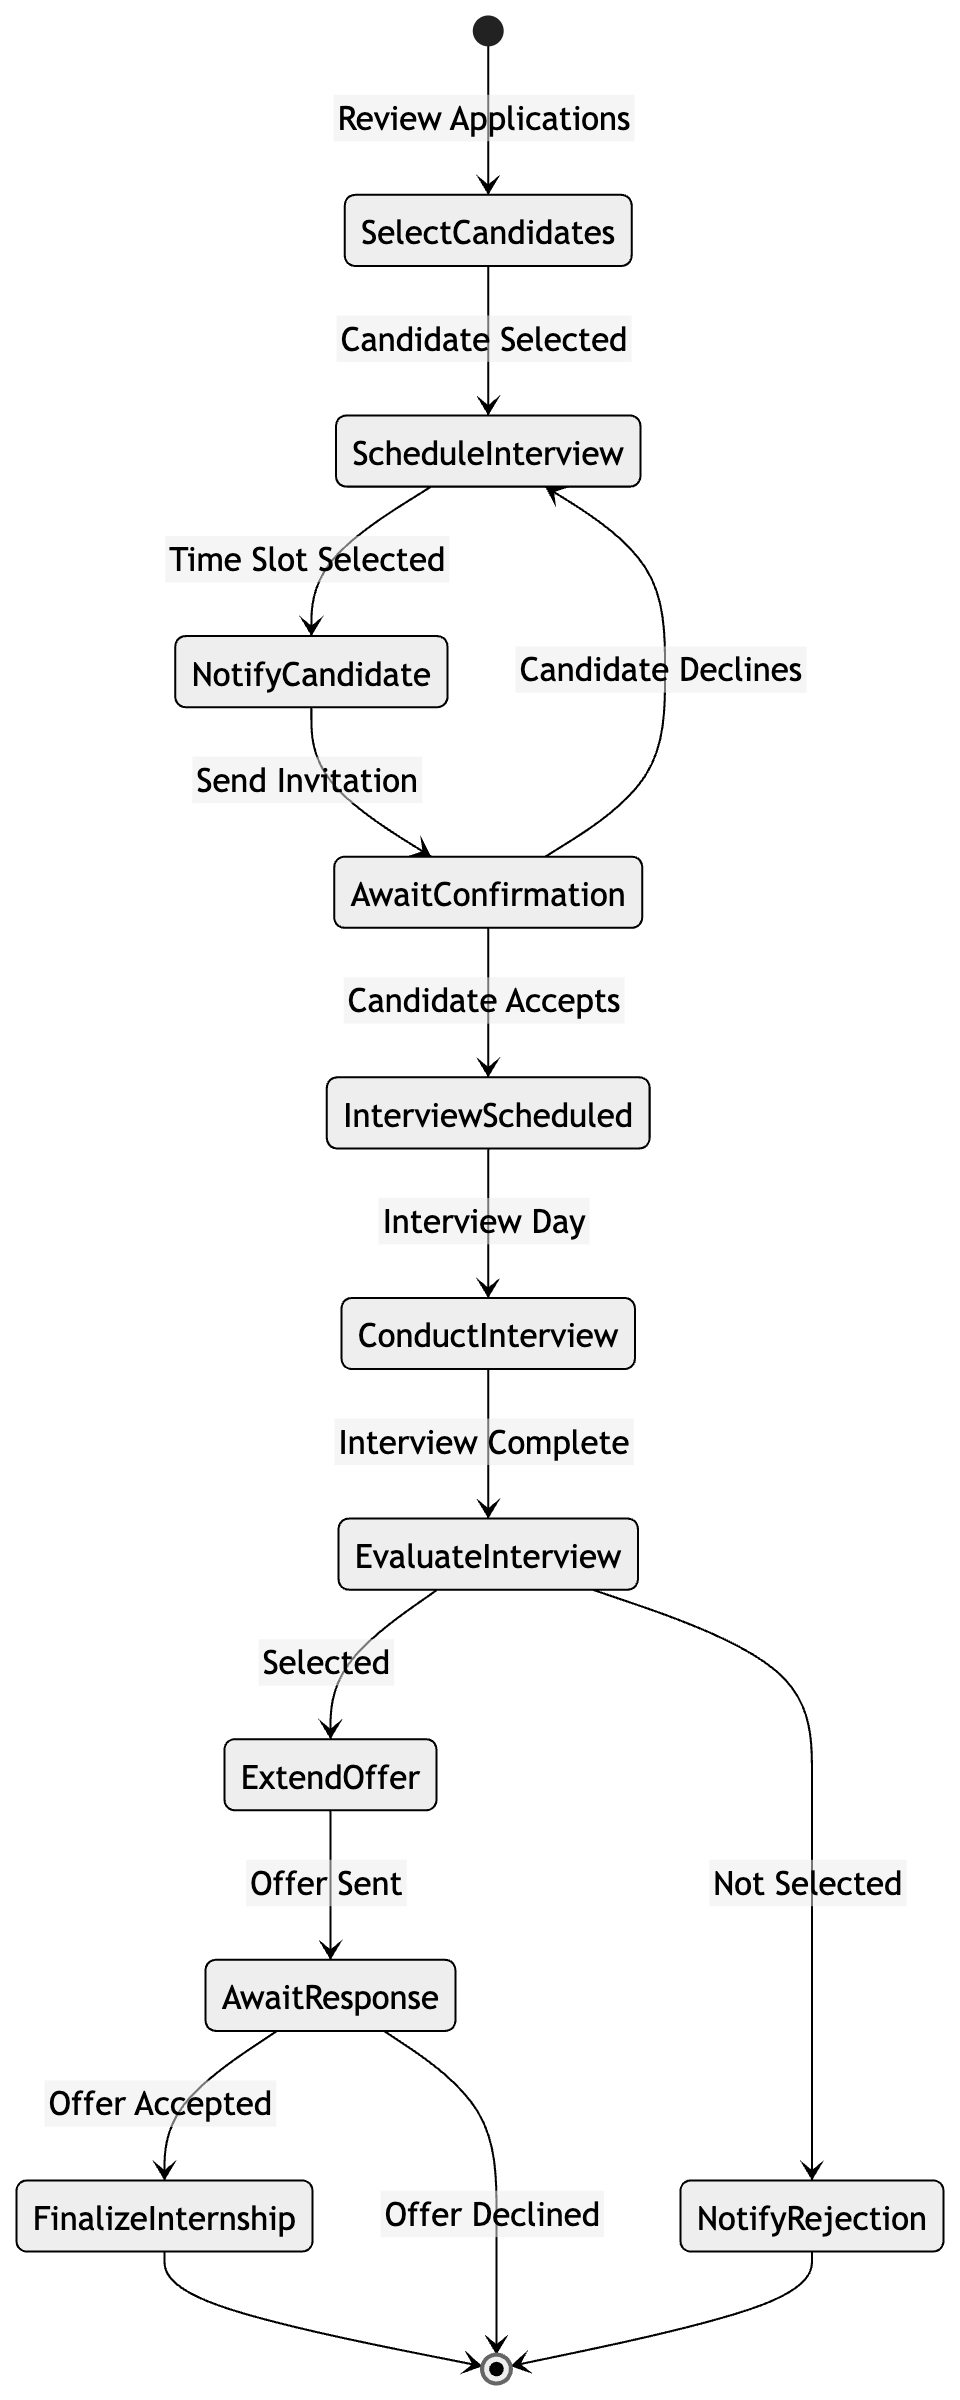
\includegraphics[width=0.45\linewidth]{JhaBhatiaSharma/Images/State Diagrams/InterviewManagement.png}
        \caption{State Diagram for Interview Management}
        \label{fig:InterviewManagement}%
    \end{center}
\end{figure}

\paragraph{Complaint Handling:}
Through S\&C, any party that experiences problems during the internship process can submit a complaint. A description of the problem and any pertinent documentation must be included in the complaint form. The relevant university official receives the complaint once it is filed. The university can look into the matter, get in touch with those involved, and try to find a solution. Every conversation and choice is recorded in the system.

\begin{figure}[H]
    \begin{center}
        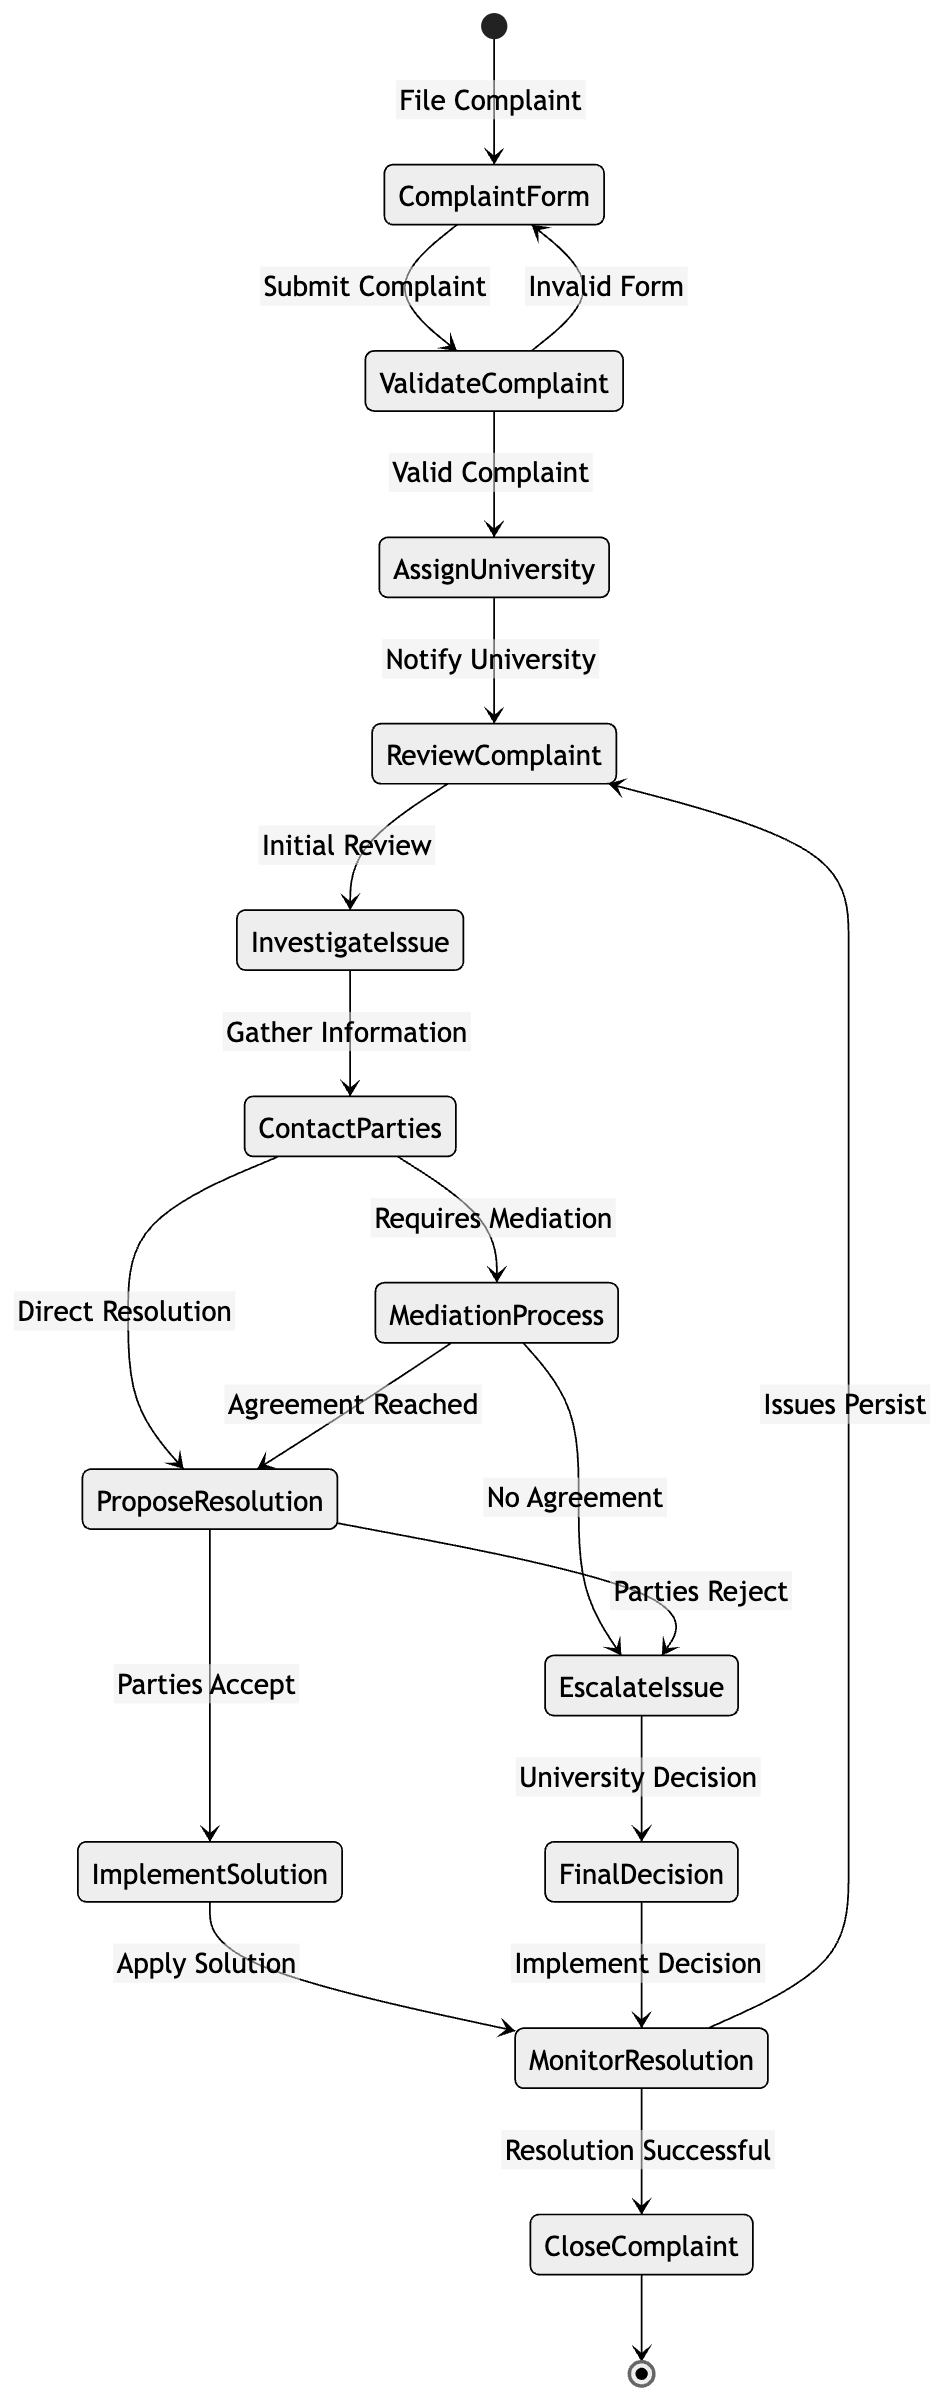
\includegraphics[width=0.42\linewidth]{JhaBhatiaSharma/Images/State Diagrams/ComplaintFiling.png}
        \caption{State Diagram for Complaint Handling}
        \label{fig:complaintHandling}%
    \end{center}
\end{figure}

\paragraph{Profile Management:}
Anytime they choose, users can view and edit their profiles. For students, this entails revising their resume, preferences, and talents. For businesses, this entails revising internship requirements and company information. S\&C verifies all modifications before they are saved. Additionally, in response to changes in profiles, the algorithm immediately updates matching recommendations.

\begin{figure}[H]
    \begin{center}
        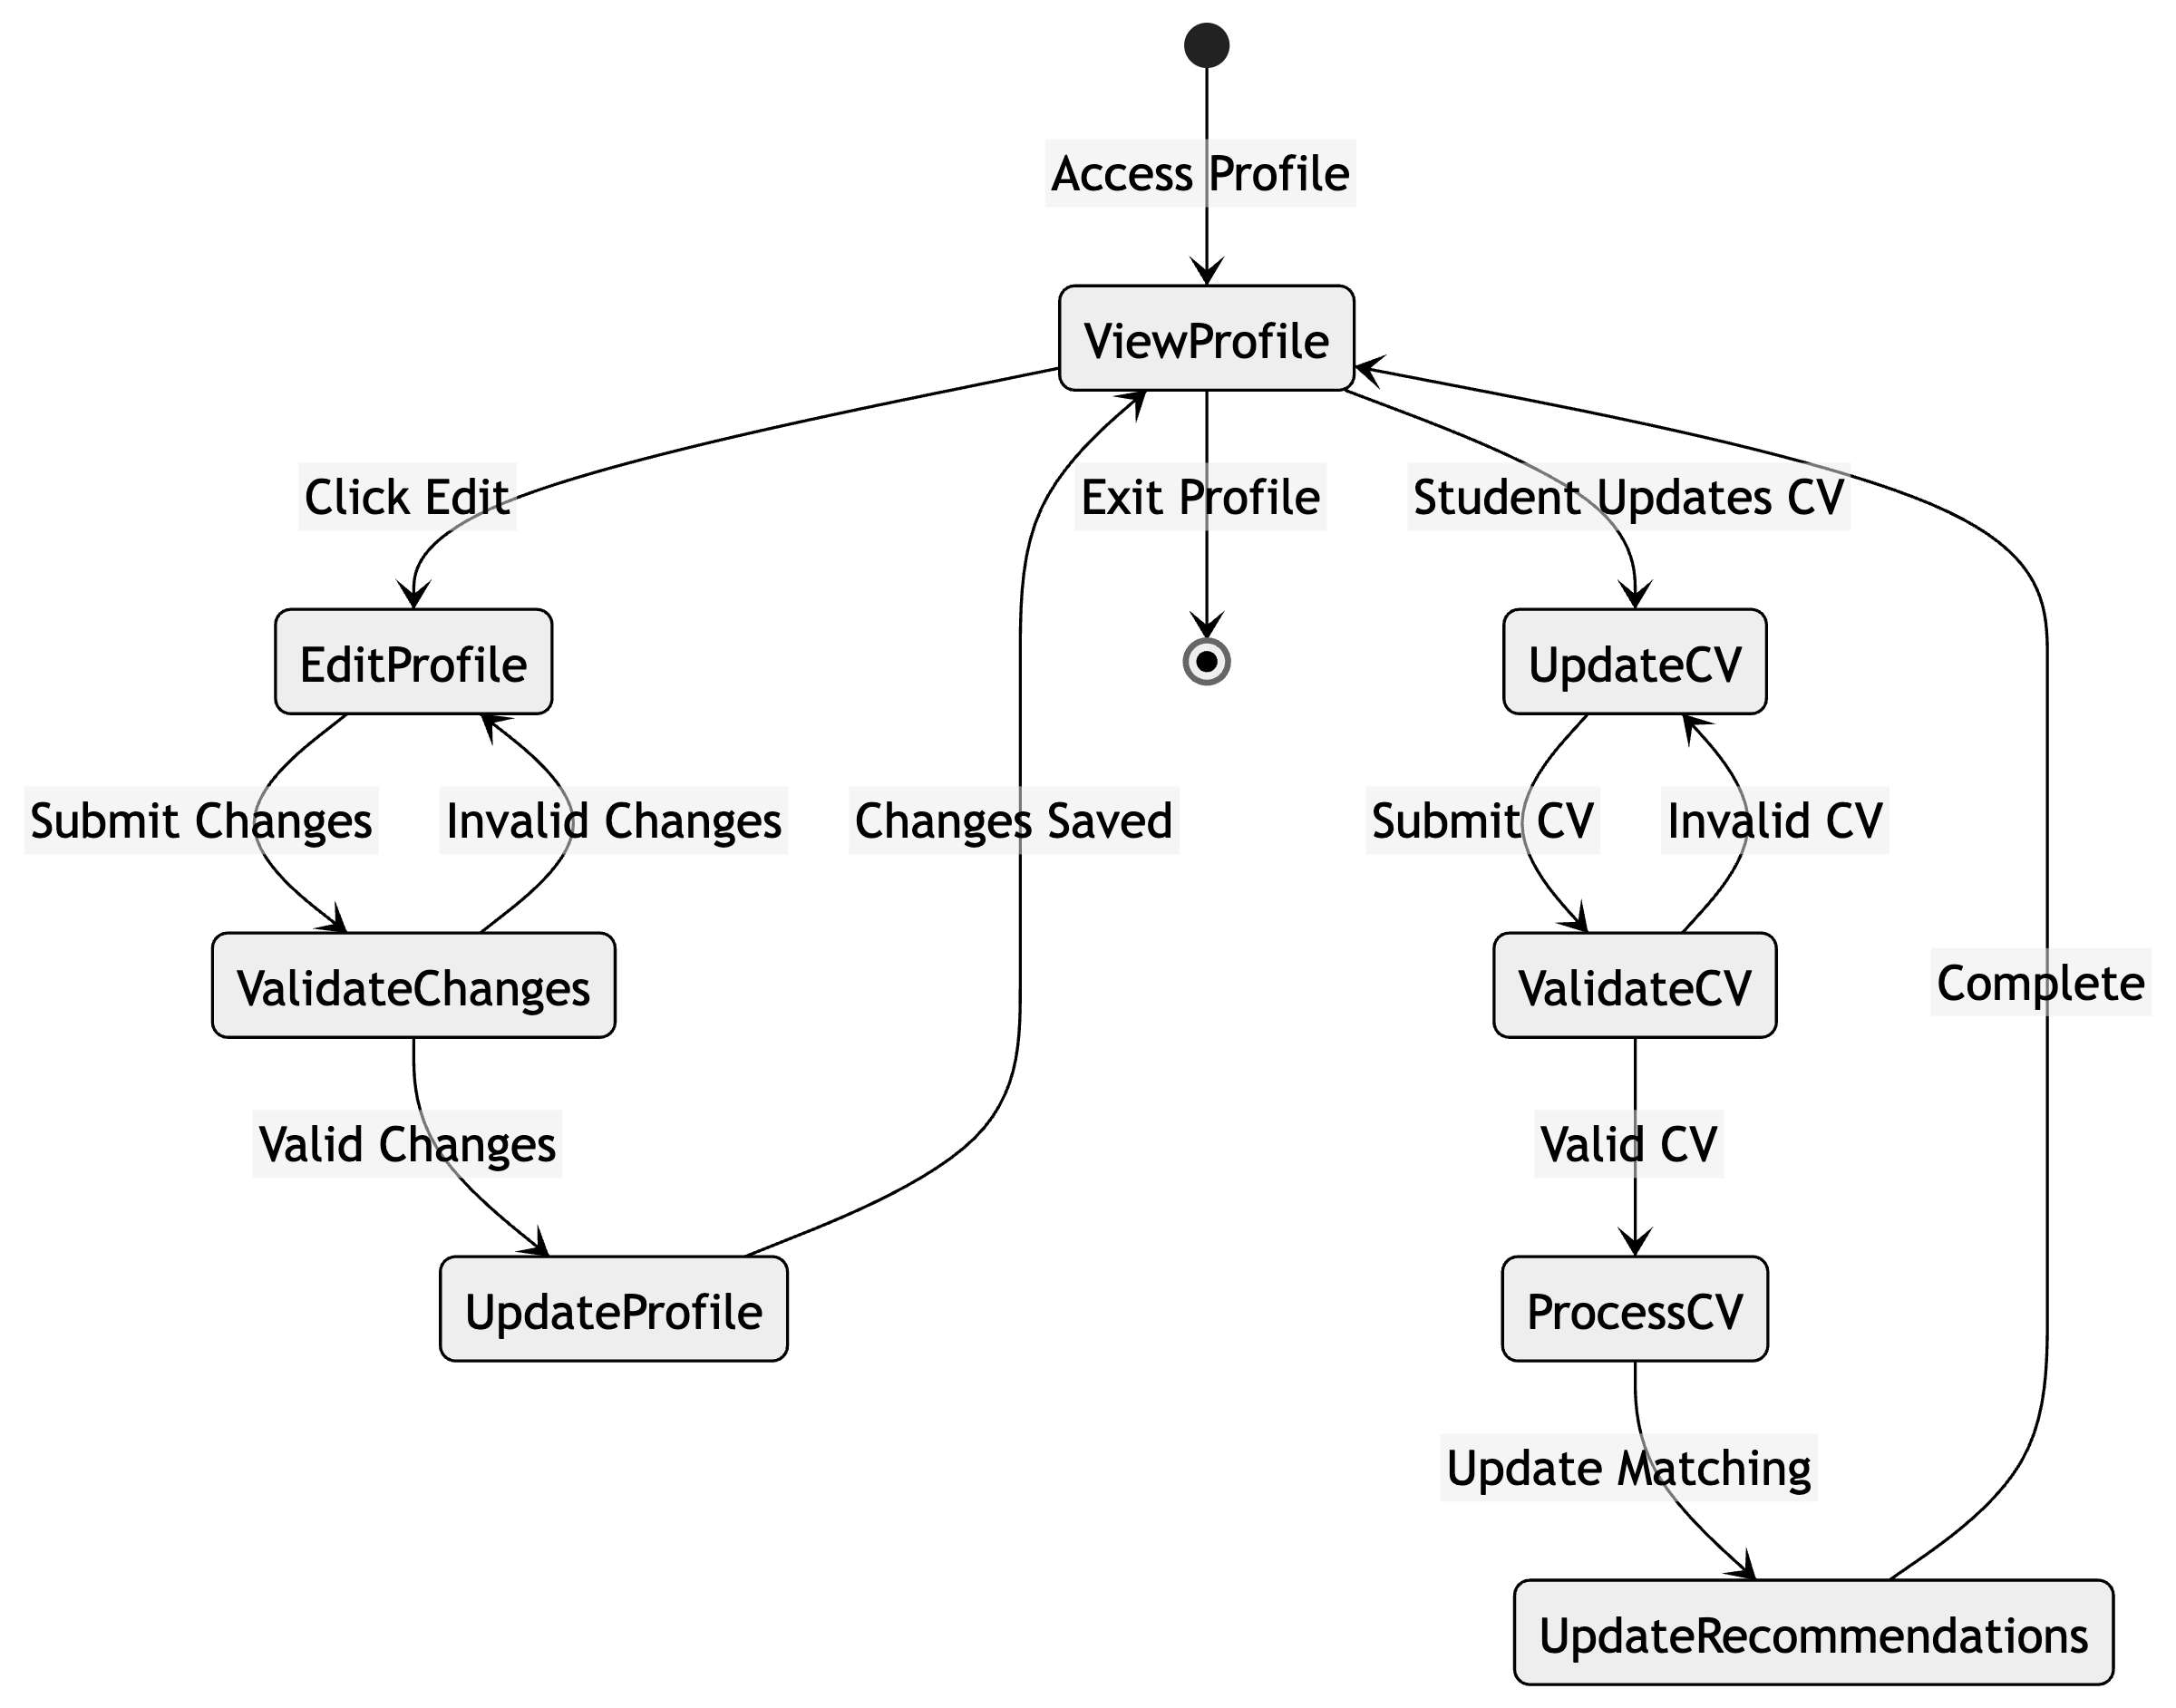
\includegraphics[width=0.8\linewidth]{JhaBhatiaSharma/Images/State Diagrams/ProfileManagement.png}
        \caption{State Diagram for Profile Management}
        \label{fig:ProfileManagement}%
    \end{center}
\end{figure}

\paragraph{Search and Filter:}
The platform's search feature allows users to look for pertinent information. Students can use industry, geography, keywords, and other parameters to find internships. Employers can look up candidate profiles by experience, education, and skill set. Additional filters can be used to further refine search results, and users can remember their search choices for later use.


\begin{figure}[H]
    \begin{center}
        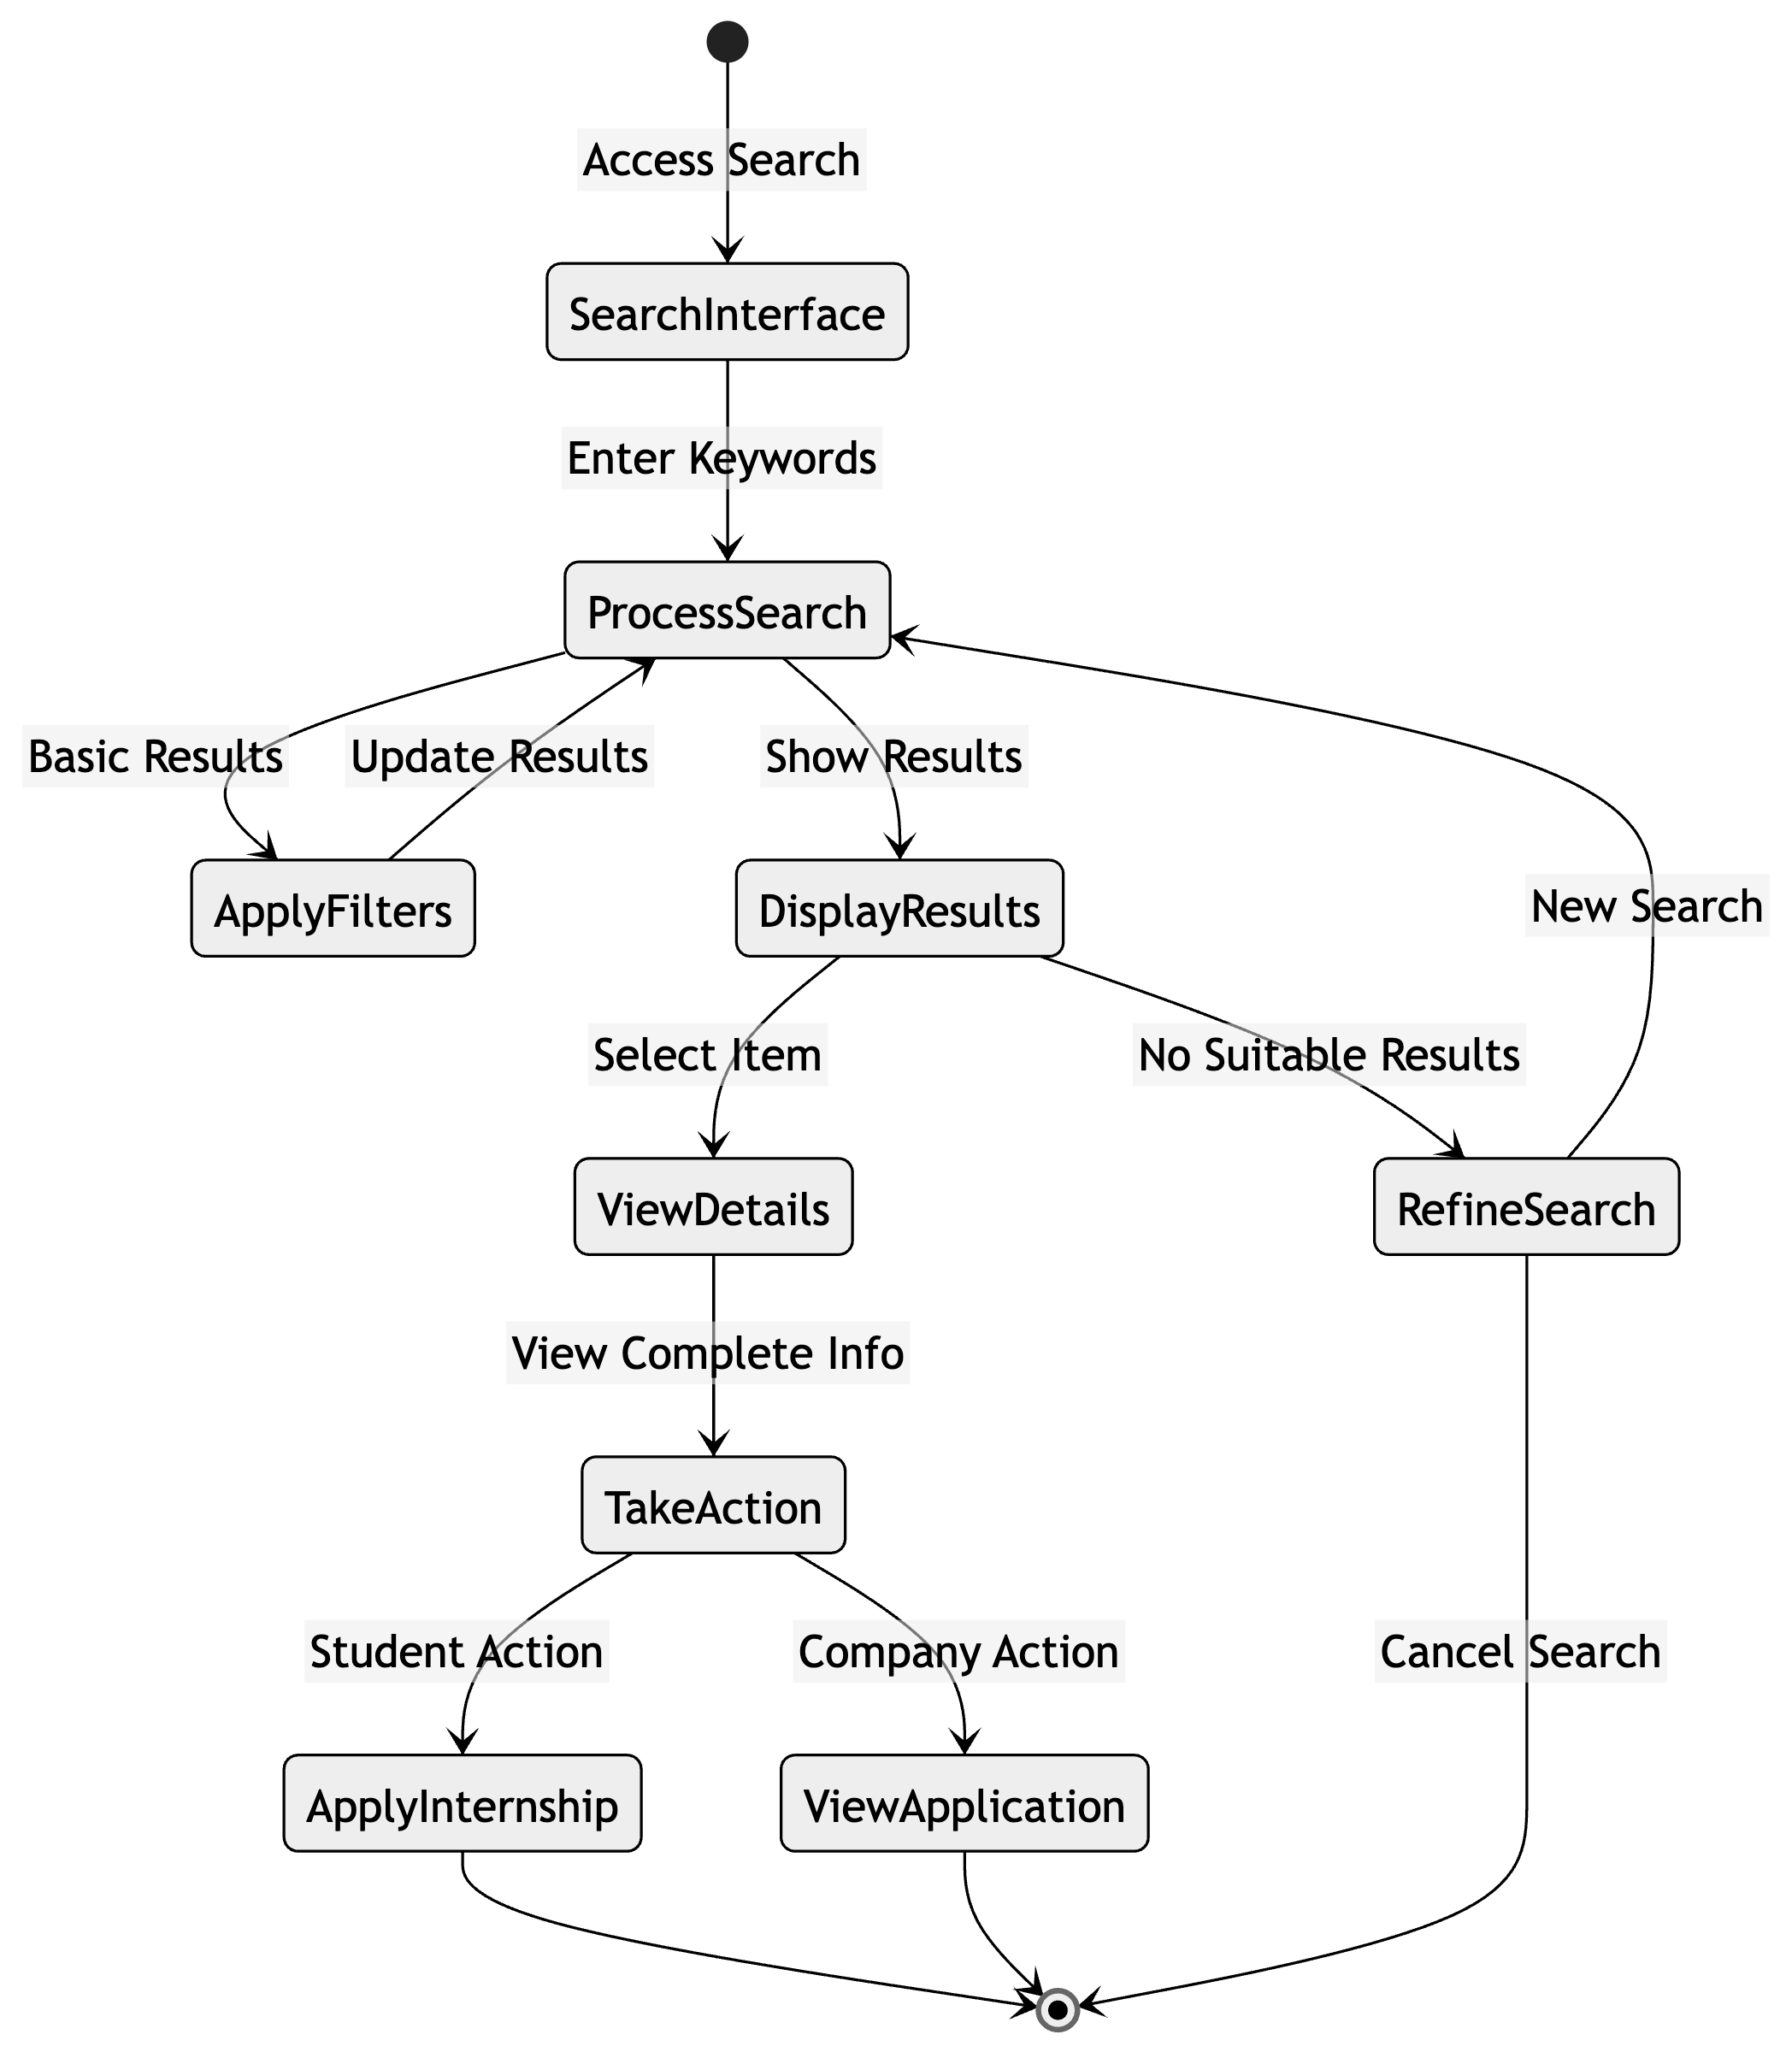
\includegraphics[width=0.6\linewidth]{JhaBhatiaSharma/Images/State Diagrams/SearchandFilter.png}
        \caption{State Diagram for Search and Filter}
        \label{fig:SearchFilter}%
    \end{center}
\end{figure}

\section{Product Functions}
\label{sec:product_functions}

\subsection{Core Functions}

\subsubsection{For Students}
\begin{itemize}
    \item \textbf{Manage Profiles and CVs:} Students can create and update their profiles, as well as submit resumes for potential employers to view.
    \item \textbf{Search and Filter Internships:} Students can use search and filtering options to find internships based on interests, location, and duration.
    \item \textbf{Monitor Applications:} Students can track the status of their internship applications and receive notifications about any changes or decisions.
    \item \textbf{Schedule Interviews:} Depending on company availability, students can select interview slots for internship positions.
    \item \textbf{Submit Feedback:} After completing an internship, students can provide feedback and comments through the platform.
    \item \textbf{File Complaints:} Students can directly lodge issues or complaints related to internships via the portal.
\end{itemize}

\subsubsection{Management of Company Profiles}
\begin{itemize}
    \item \textbf{Manage Company Profiles:} Companies can create, update, and maintain profiles containing organizational details and contact information.
    \item \textbf{Post Internships:} Companies can list internship vacancies with detailed requirements and descriptions.
    \item \textbf{Screen Candidates:} Employers can review applications and filter candidates based on their backgrounds, profiles, and other criteria.
    \item \textbf{Conduct Interviews:} Employers can schedule and conduct interviews with shortlisted candidates directly on the platform.
    \item \textbf{Gather Feedback:} Companies can give feedback on candidates after interviews or upon internship completion.
    \item \textbf{Monitor Performance:} During an intern’s tenure, employers can track the intern’s progress and performance.
\end{itemize}

\subsubsection{University Performance}
\begin{itemize}
    \item \textbf{Observe Student Activity:} Universities can monitor students’ profiles, applications, and internship progress.
    \item \textbf{Oversee Internships:} Institutions can view details of ongoing internships and assess how they align with university objectives.
    \item \textbf{Handle Complaints:} Universities are authorized to review and resolve internship-related complaints raised by students or companies.
    \item \textbf{Generate Reports:} Institutions can produce reports on internship data, student achievements, and employer feedback.
    \item \textbf{Ensure Quality Assurance:} Universities can evaluate the quality of internships to ensure they meet institutional standards.
\end{itemize}

\newpage
\section{User Characteristics}
\label{sec:User_characteristic}

\subsection{Students}
\begin{itemize}
    \item \textbf{Demographics:} University students from diverse academic backgrounds and skill levels.
    \item \textbf{Motivations:} Actively seeking internships to enhance their academic learning, gain practical experience, and develop their careers.
    \item \textbf{Technical Proficiency:} Basic computer literacy, with varying levels of technical expertise depending on their academic discipline.
    \item \textbf{Access Requirements:} Use web browsers and mobile devices for seamless access to the platform.
    \item \textbf{Engagement Needs:} Require a user-friendly interface with clear guidance for application processes, personalized internship recommendations, and progress tracking.
\end{itemize}

\subsection{Companies}
\begin{itemize}
    \item \textbf{Demographics:} Organizations ranging from startups to multinational corporations across various industries.
    \item \textbf{Key Users:}
        \begin{itemize}
            \item \textbf{HR Personnel:} Responsible for posting internships, managing candidate applications, and coordinating interviews.
            \item \textbf{Department Managers:} Assess technical and domain-specific skills of applicants.
            \item \textbf{Technical and Non-Technical Staff:} Engage with interns for mentorship and project collaboration.
        \end{itemize}
    \item \textbf{User Roles:} Flexible role-based access for different functionalities, such as job posting, candidate review, and administrative controls.
    \item \textbf{Engagement Needs:} Require tools for streamlining recruitment processes, accessing applicant analytics, and maintaining compliance with university policies.
\end{itemize}

\subsection{University Administrators}
\begin{itemize}
    \item \textbf{Key Roles:}
        \begin{itemize}
            \item \textbf{Academic Coordinators:} Oversee the alignment of internships with educational goals and curriculum requirements.
            \item \textbf{Internship Program Managers:} Monitor internship program effectiveness, gather feedback, and ensure compliance with regulations.
            \item \textbf{Student Advisors:} Guide students on selecting suitable internships and navigating application processes.
            \item \textbf{System Administrators:} Maintain the platform, manage user accounts, and ensure data security.
        \end{itemize}
    \item \textbf{Engagement Needs:} Require detailed dashboards for tracking student participation, company partnerships, and program outcomes. Need tools for generating reports and managing communications between stakeholders.
\end{itemize}

\section{Assumptions, Dependencies, and Constraints}
\label{sec:assumptions_dependencies_constraints}%

\subsection{Domain Assumptions}
\label{subsec:domain_assumptions}%
\newcounter{da}
\setcounter{da}{1}
\newcommand{\cda}{\theda\stepcounter{da}}

\begin{table}[H]
\centering
\footnotesize % Reduce font size
\begin{tabular}{ |l|p{0.75\linewidth}| }
    \hline
    \textbf{ID} & \textbf{Description} \\
    \hline
    DA\cda & Users have reliable internet access. \\
    \hline
    DA\cda & Students maintain updated CVs. \\
    \hline
    DA\cda & Companies provide accurate information about internships. \\
    \hline
    DA\cda & Universities actively monitor students' progress on S\&C. \\
    \hline
    DA\cda & All users comply with the platform's terms and policies. \\
    \hline
\end{tabular}
\caption{Domain Assumptions.}
\label{tab:domain_assumptions}
\end{table}

\subsection{Dependencies}
\label{subsec:dependencies}%
\newcounter{dep}
\setcounter{dep}{1}
\newcommand{\cdep}{\thedep\stepcounter{dep}}

\begin{table}[H]
\centering
\footnotesize
\begin{tabular}{ |l|p{0.75\linewidth}| }
    \hline
    \textbf{ID} & \textbf{Description} \\
    \hline
    D\cdep & Reliable web hosting services. \\
    \hline
    D\cdep & Functional email delivery system. \\
    \hline
    D\cdep & Secure database system. \\
    \hline
    D\cdep & File storage system for documents. \\
    \hline
    D\cdep & Authentication services to manage user logins. \\
    \hline
\end{tabular}
\caption{Dependencies.}
\label{tab:dependencies}
\end{table}

\subsection{Constraints}
\label{subsec:constraints}%
\newcounter{con}
\setcounter{con}{1}
\newcommand{\ccon}{\thecon\stepcounter{con}}

\begin{table}[H]
\centering
\footnotesize
\begin{tabular}{ |l|p{0.75\linewidth}| }
    \hline
    \textbf{ID} & \textbf{Description} \\
    \hline
    C\ccon & Must comply with GDPR and data protection regulations. \\
    \hline
    C\ccon & Adhere to university-specific internship regulations. \\
    \hline
    C\ccon & Ensure system performance under high traffic. \\
    \hline
    C\ccon & Provide compatibility across major web browsers. \\
    \hline
    C\ccon & Implement robust security standards for data handling. \\
    \hline
\end{tabular}
\caption{Constraints.}
\label{tab:constraints}
\end{table}
